\section{Implementaci\'on}
\subsection{Arquitectura de TariyKDD}
Para el desarrollo de TariyKDD se utilizaron computadores con procesador AMD 64 bits, disco duro Serial ATA,
\'util  al tomar los datos desde un repositorio y al momento de realizar pruebas de rendimiento de los
algoritmos, ya que su velocidad de transferencia es de 150 MB/sg; adem\'as la RAM que se utilizo fu\'e
superior a los 512 MB, ya que la Miner\'ia de Datos requiere grandes cantidades de memoria por el tama\~no de
los conjuntos de datos.\\
\\
El sistema operativo sobre el cual se trabajo durante la implementaci\'on de TariyKDD es Fedora Core en su
versiones 3 y 5. El lenguaje de programaci\'on en el que esta elaborado TariyKDD es Java 5.0, 
actualizaci\'on 06.\\
\\
Dentro del proceso de Descubrimiento de Conocimiento, TariyKDD comprende las etapas de Selecci\'on,
Preprocesamiento, Miner\'ia de Datos y Visualizaci\'on de Resultados. De esta forma la implementaci\'on de la
herramienta se hizo a trav\'es de los siguientes m\'odulos de software cuya estructura se muestra en la figura 7.81.

\begin{figure}[ht]
\centering
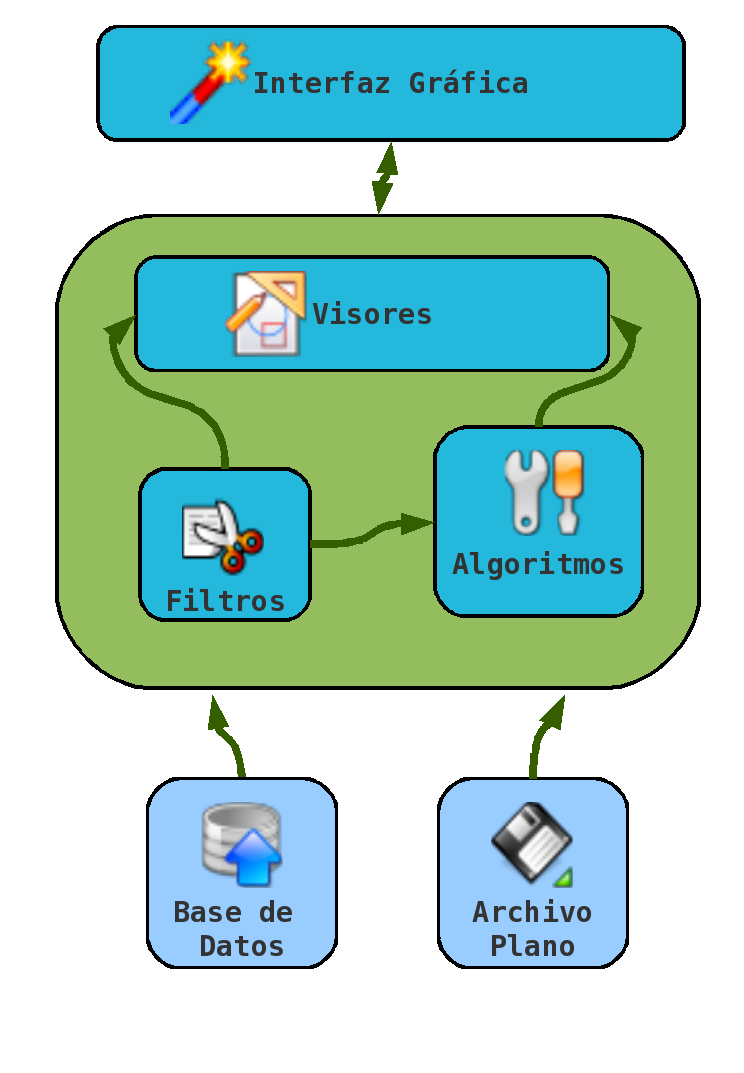
\includegraphics[width=0.5\textwidth]{images/arquitectura.png}
\caption{\'Arquitectura TariyKDD}
\end{figure}

\subsubsection{M\'odulo de Conexi\'on}
El M\'odulo de Conexi\'on permite al usuario acceder a los conjuntos de datos a trav\'es de un Archivo Plano o
una Base de Datos.\\
\\
La opci\'on Archivo Plano le permite al usuario seleccionar un conjunto de datos que se encuentra en disco, en un
archivo de acceso aleatorio, el formato para el archivo debe ser ARFF\cite{arff}, debido a que este es uno de los
m\'as conocidos y tiene una estructura que lo hace f\'acil de comprender por ser estandar (debido a su estructura
de etiquetas).\\
\\
En cuanto a la Conexi\'on a Bases de Datos, TariyKDD puede conectarse con PostgreSQL a trav\'es de su manejador
JDBC tipo 4 \cite{abcjdbc}. Este driver es el m\'as eficiente ya que traduce de forma directa las peticiones del
API Java al protocolo nativo del Sistema Gestor, con la ventaja de que resulta sencilla la migraci\'on a otro
diferente, lo \'unico que habr\'ia que hacer ser\'ia descargar el driver del fabricante adecuado.

\subsubsection{Almacenamiento de datos en memoria}
Una vez se ha hecho la conexi\'on al conjunto de datos, ya sea a trav\'es de Archivo Plano o mediante Bases de
Datos, el siguiente paso que se hace en TariyKDD es almacenar los datos en memoria principal, en una estructura
especial que admi\-nistra de manera optima el tama\~no de los datos. La cual se describe en este m\'odulo.\\
\\
Una de las principales dificultades dentro del proceso de descubrimiento de conoci\-miento es el uso adecuado de
los recursos del sistema y en especial de la memoria principal si tenemos en cuenta que se pretende trabajar con
amplios vol\'umenes de datos.  Ya sea cargando un conjunto de datos desde un archivo plano o directamente desde
una conexi\'on a un SGBD se espera organizar estos datos de una manera compacta con el objetivo de almacenar esta
informaci\'on en memoria principal evitando repetidas llamadas a disco lo que significa un aumento en los tiempos
de ejecuci\'on de la herramienta.\\
\\
Formatos tradicionales para el almacenamiento de transacciones, como el formato ARFF, trabajan con cabeceras
donde se registran los diferentes campos o atributos del conjunto de datos seguidos de las transacciones como tal,
separadas una de otra por cambios de l\'inea donde cada atributo esta separado a su vez por comas. En conjuntos de
datos discretizados cuyos atributos pueden tomar un rango determinado de valores, dentro de la parte en donde se
almacenan los datos es com\'un encontrar segmentos de transacciones que coinciden o incluso transacciones
completas que se repiten.\\
\\
Es posible aprovechar estas coincidencias dentro de una estructura de datos como un \'arbol N-Ario donde cada
rama represente una posible transacci\'on y donde las bifurcaciones dentro de esa rama representen segmentos
compartidos con otras transacciones o inclusive transacciones que est\'en contenidas dentro de esa misma rama.\\
\\
Para explicar de mejor manera esta propuesta consideremos el conjunto de datos representado en la siguiente
tabla, hay que tener en cuenta que los items del conjunto de datos original son codificados para mejorar la
administraci\'on de la memoria.\\

\begin{center}
\begin{tabular}{|c|c|c|c|c|c|c|} \hline
\textbf{T} & \textbf{A} & \textbf{B} & \textbf{C} & \textbf{D} & \textbf{E} \\ \hline
1 & 1 & 1 & 3 & 4 & 5 \\ \hline
2 & 1 & 1 & 3 & 4 & 6 \\ \hline
3 & 1 & 2 & 3 & 6 & 7 \\ \hline
4 & 2 & 3 & 4 & 1 & 3 \\ \hline
5 & 1 & 2 & 3 & 6 & 7 \\ \hline
6 & 2 & 3 & 4 & 6 & 5 \\ \hline
\end{tabular}
\end{center}

Se puede ver que los cuatro primeros campos de las transacciones 1 y 2 son iguales por lo que pueden compartir
nodos dentro del \'arbol N-Ario.\\

\begin{figure}[ht]
\centering
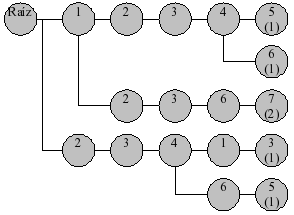
\includegraphics[width=0.5\textwidth]{images/nario2.png}
\caption{\'Arbol N-Ario}
\label{nario}
\end{figure}

Como se puede ver en la figura \ref{nario}, los valores entre par\'entesis en las hojas del \'arbol representan 
el n\'umero de repeticiones de la transacci\'on, por ejemplo la n\'umero 3 es la misma transacci\'on 5, por tanto
en el \'arbol N-Ario estos dos registros ser\'an almacenados en una sola rama, con la precauci\'on de contar su
soporte.\\
\\
Entre menos n\'umero de valores tenga un atributo y entre m\'as transacciones formen el conjunto de datos, existe
mayor posibilidad de encontrar coincidencias y aprovechar segmentos de transacciones ya almacenadas para guardar
las nuevas que se repitan.\\
\\
Un an\'alisis del presente formato para compresi\'on de datos con respecto al formato ARFF se muestra en los
anexos, en el cuadro \ref{formatos}, donde se registra el tama\~no en disco de cada formato al almacenar
conjuntos de datos con diferente n\'umero de transacciones y atributos.

\subsubsection{M\'odulo Filtros}
El m\'odulo filtros o data cleaning, se encarga de hacer un refinamiento de los datos en  dos etapas, por un lado
hace un proceso de limpieza sobre datos corruptos, vacios, ruidosos, inconsistentes, duplicados, alterados etc,
por otro lado hace una seleccion de estos datos para escojer aquellos que brinden informacion de calidad,
aplicando muestreos, discretizaciones, etc. De esta forma obtenemos datos depurados seg\'un el objetivo del
analista, para que posteriormente se pueda aplicar el nucleo KDD o de Miner\'ia de Datos sobre datos coherentes,
limpios y consistentes.\\
\\
A este m\'odulo, pertenecen los filtros de Remove Missing, Update Missing, Selection, Range, Reduction,
Codification, Replace Value, Numeric Range y Discretize, los cuales se alimentan y presentan sus resultados a
trav\'es de un TableModel que es el medio por el cual comunican sus flujos de datos.

\subsubsection{M\'odulo algoritmos}
Dentro de este m\'odulo se encuentran dos tipos de algoritmos, los de asociaci\'on y los de clasificaci\'on:

\begin{enumerate}
\item Asociaci\'on: Los algoritmos de asociaci\'on implementados en TariyKDD son EquipAsso, FPGrowth y Apriori.
Los tres algoritmos utilizan un vector de \'arboles AVL balanceados para almacenar los itemsets frecuentes. Cada
posici\'on del vector almacena un tipo de itemsets frecuentes en un \'arbol AVL. De esta forma la posici\'on 0 del
vector almacena un \'arbol AVL que contiene los itemsets frecuentes tipo 1. En este m\'odulo de TariyKDD, la mayor
ventaja que proporcionan los \'arboles AVL es la rapidez con la que se realizan las busquedas a la hora de 
determinar si un itemset frecuente ya existe.\\
\\
As\'i mismo los tres algoritmos usan el \'arbol N-Ario que se describio anteriormente para almacenar el conjunto
de datos que se vaya a minar. Los datos comprimidos en esta estructura son tomados como entradas por los tres
algoritmos, a partir de estos se aplican las t\'ecnicas de Miner\'ia de Datos correspondientes y el producto final
son las reglas.

\item Clasificaci\'on: Dentro de este m\'odulo en TariyKDD se implementaron los algoritmos Mate y C4.5. Para los
algoritmos de clasificaci\'on igual que en los de asociaci\'on la estructura que se utilizo para su 
implementaci\'on fu\'e un \'arbol N-Ario. En C4.5 y Mate para almacenar los datos en primera instancia. Ya que ha
medida que se desarrollan los algoritmos este \'arbol va cambiando, as\'i, al final el \'arbol tiene las reglas
de clasificaci\'on.\\
\\
La estructura utilizada para mostrar las reglas de clasificaci\'on es un \'arbol N-Ario que implementa los
m\'etodos de la interfaz de Java, TreeModel , la cual define un modelo de datos adecuado para poder visualizarlos
en un JTree o un control de Java que despliega las reglas jerarquicamente de acuerdo a la estructura en la que
estan almacenadas, es decir el \'arbol N-Ario.
\end{enumerate}

\subsubsection{M\'odulo Visores}
Este m\'odulo implementa las clases necesarias para mostrar de forma gr\'afica las reglas que se obtienen 
despu\'es de haber realizado Miner\'ia de Datos.\\
\\
Si el usuario ha utilizado algoritmos de asociaci\'on obtiene como resultado reglas, que puede observar a
trav\'es de una JTable, la cual es utilizada para desplegar y editar tablas de dos dimensiones. Para desplegar
estas reglas, primero, se tiene un array con los datos que se van a mostrar, a partir de estos se construye un
m\'odelo propio de tabla implementando los m\'etodos de la interfaz Java, TableModel. Des\-pu\'es simplemente el 
m\'odelo se pasa al constructor de JTable para que esta clase se encarge de desplegar las reglas.\\
\\
Pero si durante el proceso de Miner\'ia de Datos se utilizaron algoritmos de clasificaci\'on, las reglas son 
desplegadas en un \'arbol N-Ario que dentro de TariyKDD se ha llamado \'Arbol de Resultados. La construcci\'on de
este se la realiza como se dijo anteriormente implementando los m\'etodos de la interfaz TreeModel, modelo que 
luego es usado por un JTree para visualizar las reglas de manera jer\'arquica.

\subsubsection{M\'odulo GUI}

El m\'odulo de GUI es usado en los 4 m\'odulos anteriores y es el encargado de brindrar una interfaz gr\'afica amigable al usuario.  Para su desarrollo se utilizaron las funcionalidades del proyecto Matisse, proyecto encargado de proveer facilidades para la construccion de entornos gr\'aficos a los proyectos desarrollados con NetBeans y que da un soporte a las aplicaciones que usan Swing, el cual es un conjunto de clases y componentes usados en interfaces gr\'aficas desde botones hasta tablas y estructuras de \'arboles.
%%%%%%%%%%%%%%%%%%%%%%%%%%%%%%%%%%%%%%%%%%% DESCRIPCION DE CLASES %%%%%%%%%%%%%%%%%%%%%%%%%%%%%%%%%%%%%%%%%%%%%%%%
\subsection{Descripci\'on de clases}

\subsubsection{Paquete Utils}
\begin{description}
\item [Clase DataSet] En esta estructura los algoritmos de asociaci\'on almacenan los datos o items de 
forma comprimida, ocupando menos espacio en memoria. La estructura utilizada por DataSet es un \'arbol
N-Ario que almacena los datos en cada nodo como tipo short. Lo particular de esta estructura es el 
aprovechamiento de la memoria principal, ya que en una sola rama almacena items de diferentes 
transacciones, controlando individualmente su n\'umero de apariciones.
\item [Clase FileManager] Esta clase gestiona todo lo relacionado con flujos de archivos, como por 
ejemplo crear un archivo plano, construir el diccionario de datos a partir de un archivo de acceso
aleatorio, entre otras funciones.
\item [Clase BaseDatos] Esta clase gestiona todo lo relacionado con el manejo de las Bases de Datos, 
como la conexi\'on, y la selecci\'on, de atributos.
\end{description}

\begin{description}
\item [Clase NodeNoF] Esta clase representa un nodo b\'asico del DataSet, este nodo no tiene soporte.
\item [Clase NodeF] Esta clase extiende a la clase NodeF y agrega el soporte a cada nodo del DataSet.
\item [Clase AvlTree] Los itemsets frecuentes generados por los algoritmos de asociaci\'on son
almacenados en un \'arbol AVL balanceado, cuya estructura se encuentra en esta clase.
\item [Clase AvlNode] Es en si, un nodo del \'arbol AVL que almacena los itemsets frecuentes. Tiene un
campo de tipo ItemSet en donde se guarda el dato que va en el nodo y tiene los punteros derecho e 
izquierdo a los dem\'as nodos del \'arbol.
\item [Clase ItemSet] La clase ItemSet almacena un conjunto de items o itemsets en un vector as\'i como
su respectivo soporte.
\item [Clase Transaction] Esta clase gestiona todas las operaciones que deben hacerse sobre las
transacciones. Como por ejemplo cargar las transacciones para los diferentes algoritmos y as\'i como 
tambi\'en realiza los diferentes ordenamientos de las transacciones, por item y por soporte.
\end{description}

\subsubsection{Paquete Apriori}
\begin{description}
\item [Clase Apriori] Esta clase implementa todos los m\'etodos necesarios para ejecutar el algoritmo Apriori. Los
parametros necesarios para comenzar el algoritmo son: un soporte de tipo short y un dataset (estructura de tipo
\'arbol N-Ario en la cual los datos son comprimidos) y sobre el cual se realizan tantos recorridos como itemsets
frecuentes existan.
\end{description}

\subsubsection{Paquete EquipAsso}
\begin{description}
\item [Clase EquipAsso] Para ejecutar el algoritmo EquipAsso los parametros necesa\-rios son: un soporte de tipo
short y un dataset (estructura de tipo \'arbol N-Ario en la cual los datos son comprimidos). Basicamente para
obtener los itemsets frecuentes, lo primero que se debe hacer es recorrer el \'arbol N-Ario tomar cada una de
sus transacciones, realizar todas sus combinaciones y ver cual de ellas pasa soporte y clasifica como itemset
frecuente.
\item [Clase Combinations] Recibe como parametros el tipo y el itemset a combinar. El tipo es un n\'umero que
indica hasta que profundidad se desea combinar el itemset en cuestion.
\end{description}

\subsubsection{Paquete FPGrowth}
\begin{description}
\item [Clase FPGrowth] El algoritmo FPGrowth tiene su propio \'arbol N-Ario para almacenar los datos. Recorre el
\'arbol y toma cada una de sus ramas, a partir de estas construye los Patrones Condicionales Base, luego los
Patrones Condicionales y a partir de estos determina cuales son los itemsets frecuentes, los cuales se almacenan en
un \'arbol AVL balanceado.
\item [Clase FPGrowthNode] Clase que tiene la estructura del \'arbol N-Ario del algoritmo FPGrowth. Es decir tiene
los punteros necesarios para armar un \'arbol N-Ario, tiene un puntero al hijo, al padre y al hermano.
\item [Clase BaseConditional] Clase que almacena los Patrones Condicionales Base a partir del \'arbol N-Ario de la 
clase FPGrowth.
\item [Clase BaseConditonals] Solo los nodos que pasan el soporte min\'imo se consi\-deran frecuentes, estos, tienen
un puntero a cada uno de sus Patrones Condicionales Base, a partir de los cuales se obtienen los itemsets
frecuentes.
\end{description}

\subsubsection{Paquete MateBy}
\begin{description}
\item [Clase MateBy] As\'i como los dem\'as algoritmos, MateBy utiliza el dataset o estructura de tipo
\'arbol N-Ario para comprimir los datos que se van a minar. A partir de estos datos se realizan
combinaciones y se calcula su entrop\'ia y su ganancia. Las combinaciones con la mayor ganancia se
almacenan en un \'arbol de reglas, conformando as\'i los resultados de MateBy.
\item [Clase Entro] Agrupa los nodos del \'arbol de acuerdo a su padre o rama y determina quienes tienen
la mayor ganancia, de acuerdo a esto se construye el \'arbol de reglas.
\end{description}

%%%%%%%%%%%%%%%%%%%%%%%%%%%%CASOS DE USO REALES%%%%%%%%%%%%%%%%%%%%%%%%%%%%%%%%%%%%%%%%%%%%%%%%
\newpage
\subsection{Casos de uso reales}
\subsubsection{Ingreso a la aplicaci\'on}
\begin{figure}[ht]
\centering
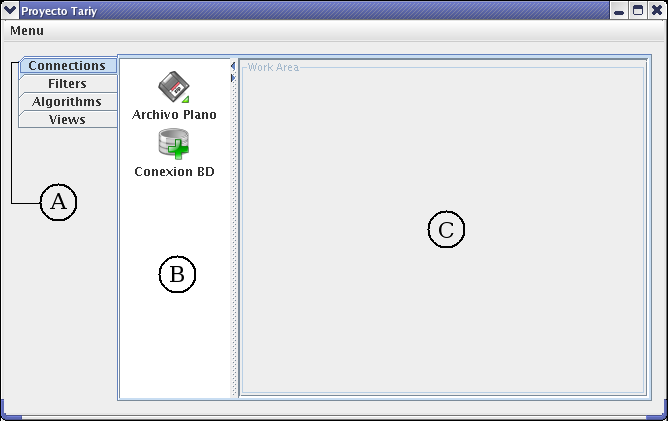
\includegraphics[width=1\textwidth]{images/01.png}
\caption{Ingreso a la aplicaci\'on}
\end{figure}
% TABLA 1
\begin{center}
\begin{tabular}{|p{60mm}|p{60mm}|} \hline
ACCI\'ON DEL ACTOR & RESPUESTA DEL SISTEMA \\ \hline
1. El usuario ejecuta la aplicaci\'on & 2. La interfaz gr\'aica de la aplicaci\'on aparece como se muestra en la figura. A: \'Area de pesta\~nas a trav\'es de las cuales se puede acceder a los difernetes m\'odulos de la aplicaci\'on. Ej, el m\'oulo por defecto es `Connections`. B: \'Area en la que aparecen las opciones de cada m\'odulo. Ej, las opciones del m\'odulo 'Connections' son 'Archivo Plano' y 'Conexi\'on DB'.   C: \'Area de trabajo sobre la que se arman los proyectos de Miner\'ia de Datos\\ \hline
\end{tabular}
\end{center}
\newpage
\subsubsection{M\'odulo filtros}
\begin{figure}[ht]
\centering
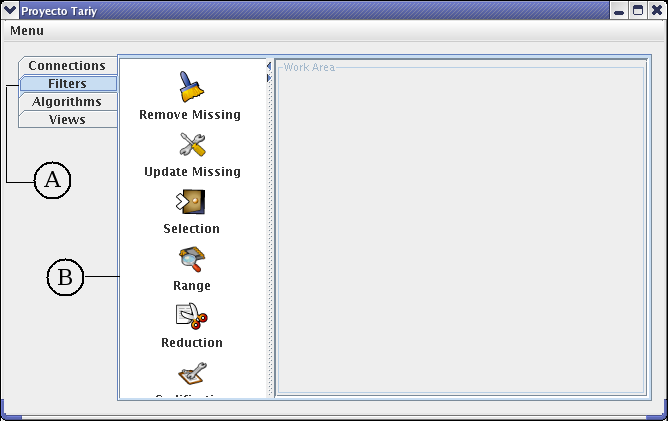
\includegraphics[width=1\textwidth]{images/02.png}
\caption{M\'odulo filtros}
\end{figure}
% TABLA 2
\begin{center}
\begin{tabular}{|p{60mm}|p{60mm}|} \hline
ACCI\'ON DEL ACTOR & RESPUESTA DEL SISTEMA \\ \hline
1. El usuario hace click en la pesta\~na A 'Filtros' & 2. Aparecen B Las opciones del m\'odulo 'Filtros'\\ \hline
\end{tabular}
\end{center}

\newpage
\subsubsection{M\'odulo algoritmos}
\begin{figure}[ht]
\centering
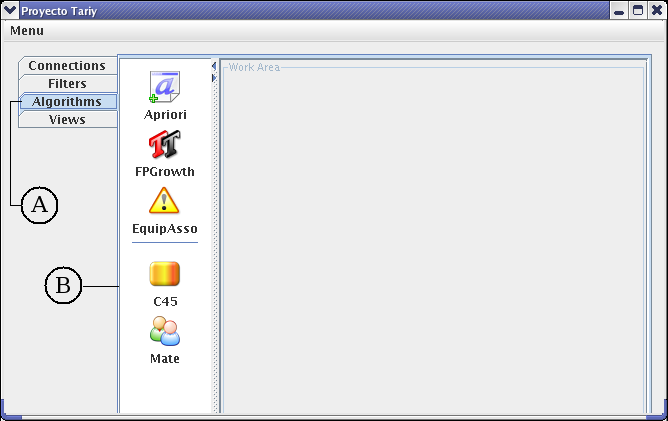
\includegraphics[width=1\textwidth]{images/03.png}
\caption{M\'odulo algoritmos}
\end{figure}
% TABLA 3
\begin{center}
\begin{tabular}{|p{60mm}|p{60mm}|} \hline
ACCI\'ON DEL ACTOR & RESPUESTA DEL SISTEMA \\ \hline
1. El usuario hace click en la pesta\~na A 'Algoritmos' & 2. Aparecen B Las opciones del m\'odulo 'Algoritmos' \\ \hline
\end{tabular}
\end{center}

\newpage
\subsubsection{M\'odulo visualizaci\'on}
\begin{figure}[ht]
\centering
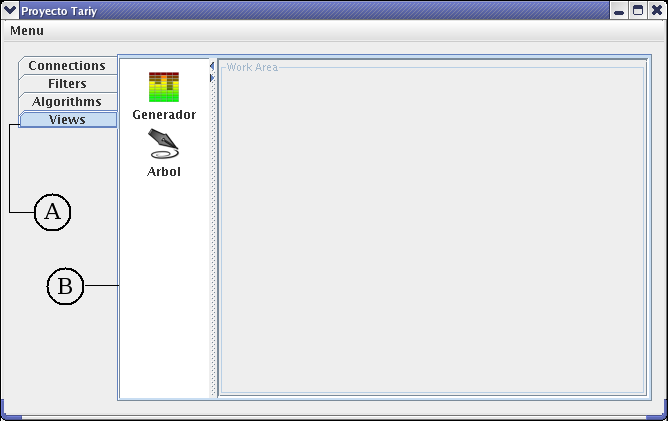
\includegraphics[width=1\textwidth]{images/04.png}
\caption{M\'odulo visualizaci\'on}
\end{figure}
% TABLA 4
\begin{center}
\begin{tabular}{|p{60mm}|p{60mm}|} \hline
ACCI� DEL ACTOR & RESPUESTA DEL SISTEMA \\ \hline
1. El usuario hace click en la pesta\~na A 'Visualizaci\'on' & 2. Aparecen B Las opciones del m\'odulo 'Visualizaci\'on' \\ \hline
\end{tabular}
\end{center}

\newpage
\subsubsection{Conexi\'on a un archivo plano}
\begin{figure}[ht]
\centering
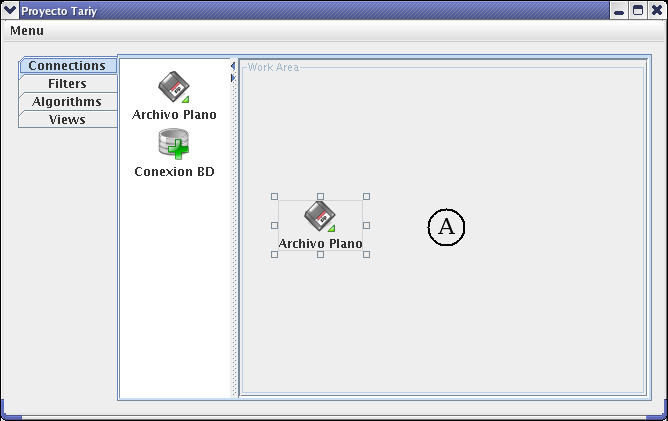
\includegraphics[width=1\textwidth]{images/05.png}
\caption{Conexi\'on a un archivo plano}
\end{figure}
% TABLA 5
\begin{center}
\begin{tabular}{|p{60mm}|p{60mm}|} \hline
ACCI\'ON DEL ACTOR & RESPUESTA DEL SISTEMA \\ \hline
1. El usuario hace click sobre el \'icono 'Archivo de Texto' & 2. El \'icono 'Archivo de Texto' aparece sobre A: \'area de trabajo.\\ \hline
\end{tabular}
\end{center}

\newpage
\subsubsection{Conexi\'on a una base de datos}
\begin{figure}[ht]
\centering
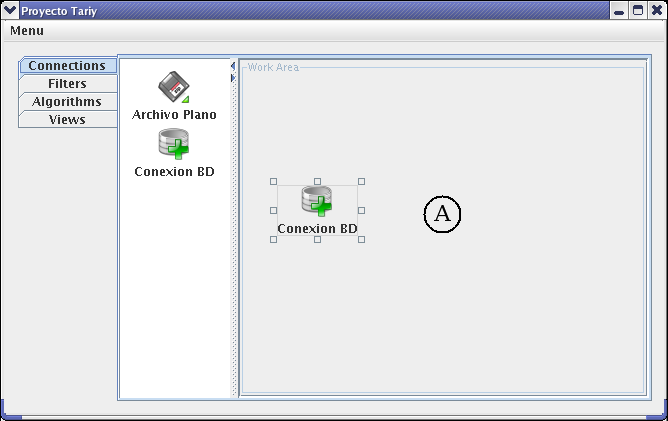
\includegraphics[width=1\textwidth]{images/06.png}
\caption{Conexi\'on a una base de datos}
\end{figure}
% TABLA 6
\begin{center}
\begin{tabular}{|p{60mm}|p{60mm}|} \hline
ACCI\'ON DEL ACTOR & RESPUESTA DEL SISTEMA \\ \hline
1. El usuario hace click sobre el \'icono 'Conexi\'on BD' & 2. El \'icono 'Conexi\'on BD' aparece sobre A: \'area de trabajo.\\ \hline
\end{tabular}
\end{center}

\newpage
\subsubsection{Men\'u emergente conexi\'on BD}
\begin{figure}[ht]
\centering
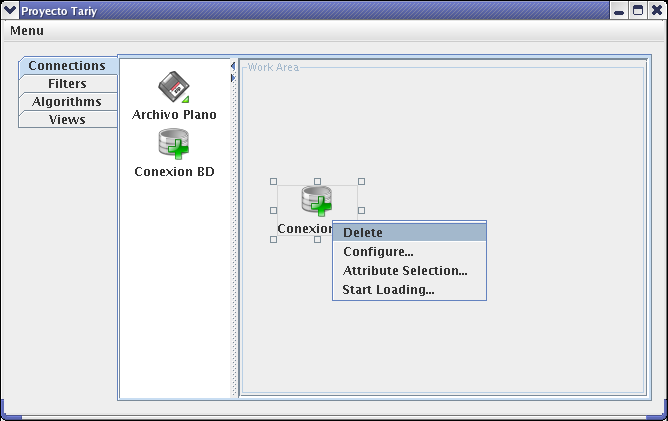
\includegraphics[width=1\textwidth]{images/07.png}
\caption{Men\'u emergente conexi\'on BD}
\end{figure}
% TABLA 7
\begin{center}
\begin{tabular}{|p{60mm}|p{60mm}|} \hline
ACCI� DEL ACTOR & RESPUESTA DEL SISTEMA \\ \hline
1. El usuario hace click derecho sobre el \'icono 'Conexi\'on BD' & 2. Se depliega A: menu del \'icono 'Conexi\'on BD'. Las opciones son: 'Delete': usada para eliminar el \'icono del \'area de trabajo. 'Configure': usada para configurar la conexi\'on a una base de datos. 'Selecci\'on de atributos': usada para seleccionar de forma gr\'afica los datos que ser\'ia usados m\'as adelante. 'Cargar': ejecuta el query que se gener\'a en la selecci\'on de atributos\\ \hline
\end{tabular}
\end{center}

\newpage
\subsubsection{Configuraci\'on conexi\'on BD}
\begin{figure}[ht]
\centering
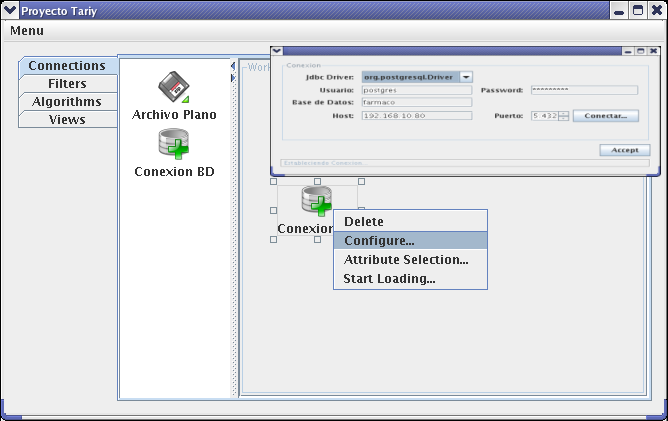
\includegraphics[width=1\textwidth]{images/08.png}
\caption{Configuraci\'on conexi\'on BD}
\end{figure}
% TABLA 8
\begin{center}
\begin{tabular}{|p{60mm}|p{60mm}|} \hline
ACCI\'ON DEL ACTOR & RESPUESTA DEL SISTEMA \\ \hline
1. El usuario hace click derecho sobre el \'icono 'Conexi\'on BD' y selecciona la opci\'on 'Configure'  & 2. Emerge una ventana de configuraci\'on de conexi\'on a bases de datos\\ \hline
\end{tabular}
\end{center}


\newpage
\subsubsection{Ventana de conexi\'on BD}
\begin{figure}[ht]
\centering
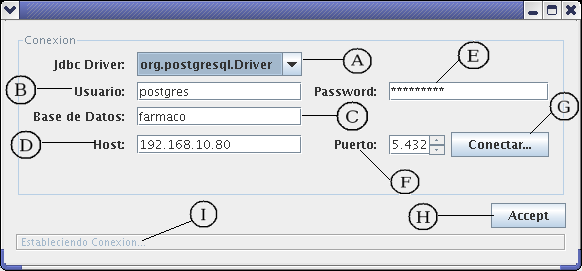
\includegraphics[width=1\textwidth]{images/11.png}
\caption{Ventana de conexi\'on BD}
\end{figure}
% TABLA 8
\begin{center}
\begin{tabular}{|p{60mm}|p{60mm}|} \hline
ACCI\'ON DEL ACTOR & RESPUESTA DEL SISTEMA \\ \hline
1. El usuario desea configurar la conexi\'on a una base de datos'  & 2. Las opciones de la ventana de configuraci\'on de conexi\'on a bases de datos tiene los siguientes campos: A: Lista de controladores ODBC para varios tipos de bases de datos. B: Nombre del usuario de la base de datos. C: Nombre de la base de datos. D: Nombre del servidor. E: 'Password': clave de acceso a la base de datos. F: nmero del puerto utilizado para la comunicaci\'on con la base de datos. G: bot\'on de conexi\'on. H: bot\'on para aceptar la conexi\'on hecha. I: mensaje que indica el estado de la conexi\'on. \\ \hline
\end{tabular}
\end{center}

\newpage
\subsubsection{Selecci\'on de atributos}
\begin{figure}[ht]
\centering
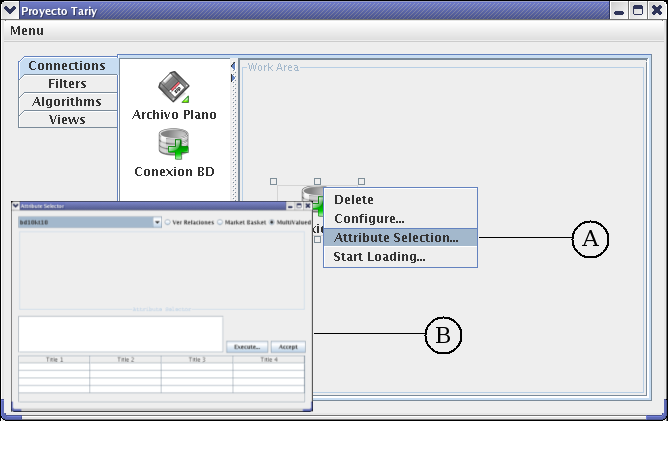
\includegraphics[width=1\textwidth]{images/09.png}
\caption{Selecci\'on de atributos}
\end{figure}
% TABLA 8
\begin{center}
\begin{tabular}{|p{60mm}|p{60mm}|} \hline
ACCI\'ON DEL ACTOR & RESPUESTA DEL SISTEMA \\ \hline
1. El usuario hace click derecho sobre el \'icono 'Conexi\'on BD' para hacer la selecci\'on de atributos  & 2. Aparece el men\'u emergente del \'icono.y se ejecuta la ventana de selecci\'on de atributos A. \\ \hline 3. El usuario hace click en la opci\'on B: 'Selecci\'on de Atributos' & 4. Aparece la ventana de selecci\'on de atributos B.  \\ \hline
\end{tabular}
\end{center}

\newpage
\subsubsection{Ventana selecci\'on de atributos}
\begin{figure}[ht]
\centering
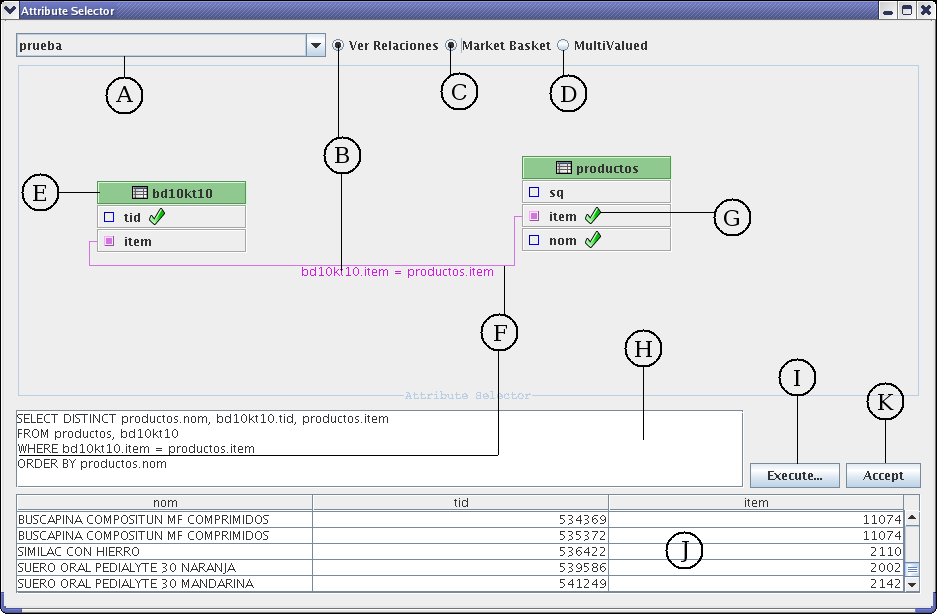
\includegraphics[width=1\textwidth]{images/attverMark.png}
\caption{Ventana selecci\'on de atributos}
\end{figure}
% TABLA 8
\begin{center}
\begin{tabular}{|p{60mm}|p{60mm}|} \hline
ACCI\'ON DEL ACTOR & RESPUESTA DEL SISTEMA \\ \hline
1. El usuario desea hacer la selecci\'on de atributos  & 2. Aparece la ventana de selecci\'on de atributos. A: lista desplegable de las tablas de la base de datos a la que se ha conectado. Al seleccionar una de ellas su representaci\'on gr\'afica aparecera en el espacio de trabajo E. B: opci\'on que permite ver las relaciones establecidas a trav\'es de la l\'inea de conexi\'on de atributos entre las tablas. C: esta opci\'on es \'util cuando se trabajan problemas de canasta de mercado. D: opci\'on para trabajar tablas multivaluadas. F:l\'inea que permite realizar las relaciones entre atributos de dos tablas. El resultado de la relaci\'on establecida se refleja en el query. G:Si se hace click sobre uno de los atributos aparece un \'icono de verificaci\'on que indica los campos que ser\'an mostrados al ejecutar el query. H: espacio en el que se crea el query. Es posible editarlo manualmente. I: bot\'on de ejecuci\'on del query. J: tabla en la que se muestra el resultado de la ejecuci\'on del query. K: bot\'on para aceptar las operaciones realizadas.   \\ \hline
\end{tabular}
\end{center}

\newpage
\subsubsection{Filtro Remove Missing}
\begin{figure}[ht]
\centering
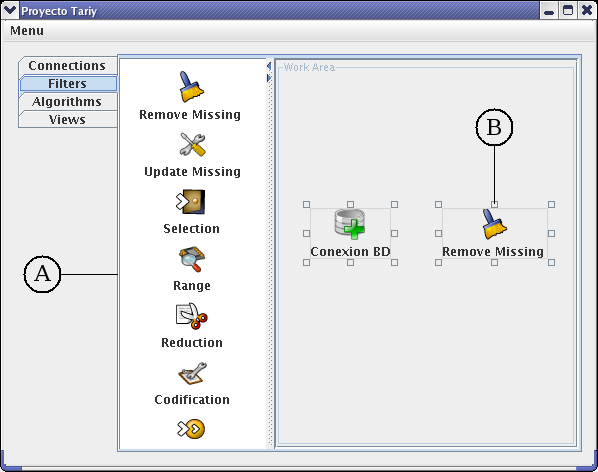
\includegraphics[width=1\textwidth]{images/17.png}
\caption{Filtro Remove Missing}
\end{figure}
% TABLA 12
\begin{center}
\begin{tabular}{|p{60mm}|p{60mm}|} \hline
ACCI\'ON DEL ACTOR & RESPUESTA DEL SISTEMA \\ \hline
1. El usuario hace click sobre uno de los \'iconos del m�ulo A: 'Filtros'.   & 2. En el \'area de opciones del m\'odulo aparecen los 9 \'iconos correspondientes a los filtros\\ \hline
3. El usuario hace click sobre uno de los \'iconos correspondientes a los filtros. & 4. El \'icono correspondiente aparace en el \'area de trabajo B.\\ \hline
\end{tabular}
\end{center}

\newpage
\subsubsection{Conexi\'on filtros a BD}
\begin{figure}[ht]
\centering
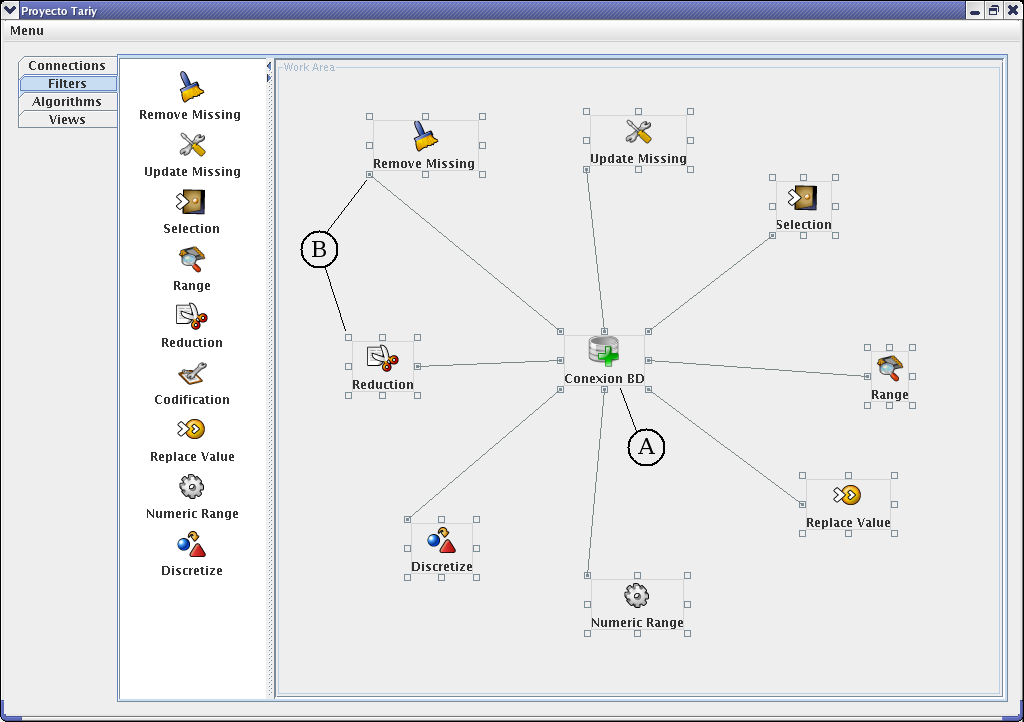
\includegraphics[width=1\textwidth]{images/19.png}
\caption{Conexi\'on filtros a BD}
\end{figure}
% TABLA 12
\begin{center}
\begin{tabular}{|p{60mm}|p{60mm}|} \hline
ACCI\'ON DEL ACTOR & RESPUESTA DEL SISTEMA \\ \hline
1. El usuario conecta una base de datos a alguno o varios de de los filtros A. & 2. Los \'iconos pueden ser conectados por medio de una l\'inea B.\\ \hline
\end{tabular}
\end{center}

\newpage
\subsubsection{Men\'u emergente de filtros}
\begin{figure}[ht]
\centering
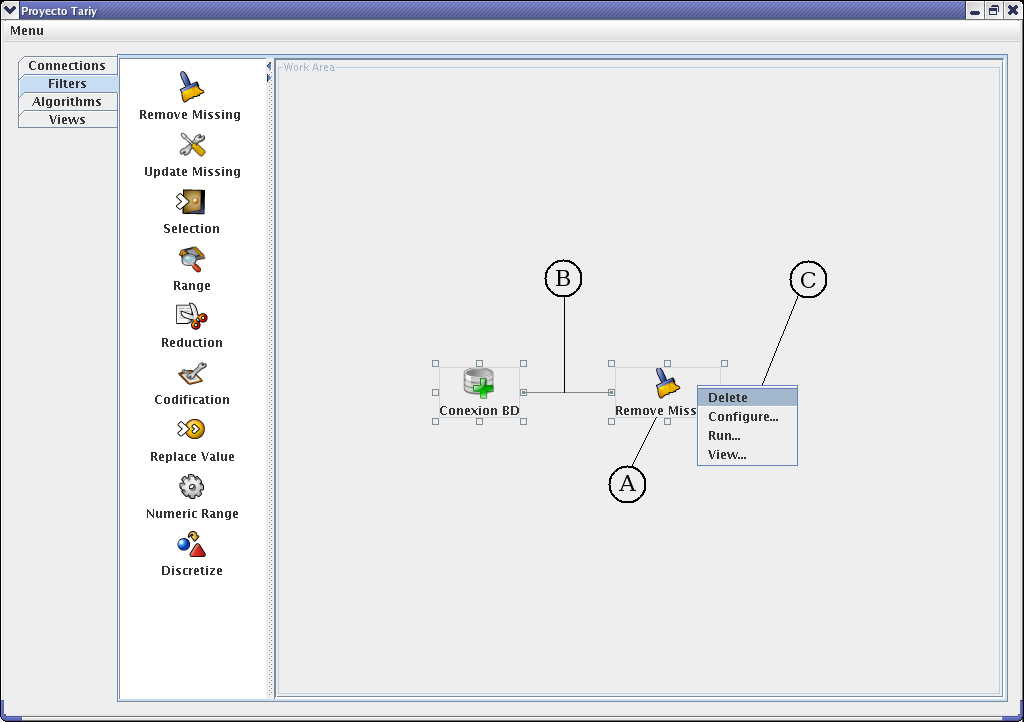
\includegraphics[width=1\textwidth]{images/f1.png}
\caption{Men\'u emergente de filtros}
\end{figure}
% TABLA 13
\begin{center}
\begin{tabular}{|p{60mm}|p{60mm}|} \hline
ACCI\'ON DEL ACTOR & RESPUESTA DEL SISTEMA \\ \hline
1. El usuario hace click sobre el \'icono 'Remove Missing'. & 2. El \'icono aparece en el \'area de trabajo A.\\ \hline
3. El usuario conecta el filtro a la base de datos. & 4. Aparece un hilo que conecta los \'iconos B.\\ \hline
5. EL usuario hace click derecho sobre el filtro. & 6. Aparece el menu emergente del \'icono C. La opci\'on Delete, borra el filtro del \'area de trabajo. Este filtro no tiene ventana de configuraci\'on. La opci\'on 'Run' ejecuta la aplicaci\'on del filtro. La opci\'on 'View' muestra la ventana de vizualizaci\'on de datos que ser\'ia descrita en el siguiente caso de uso\\ \hline
\end{tabular}
\end{center}

\newpage
\subsubsection{Visualizaci\'on de datos filtrados}
\begin{figure}[ht]
\centering
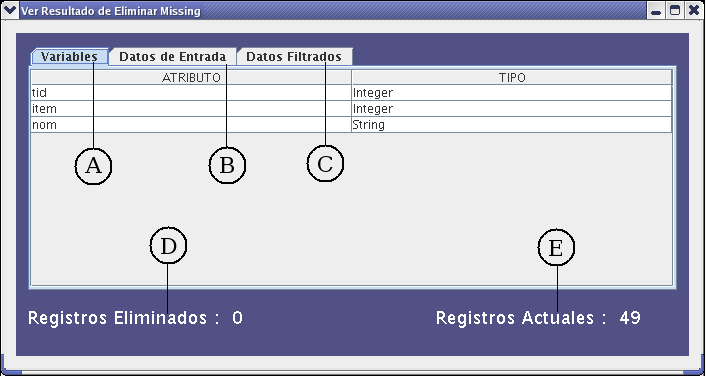
\includegraphics[width=0.8\textwidth]{images/fv1.png}
\caption{Visualizaci\'on de datos filtrados}
\end{figure}
\begin{figure}[ht]
\centering
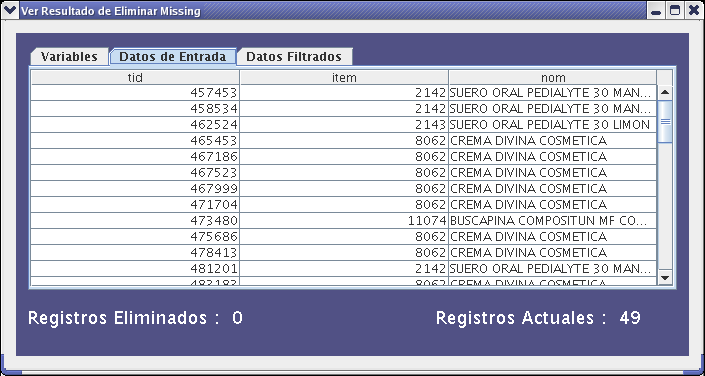
\includegraphics[width=0.7\textwidth]{images/fv2.png}
\caption{caso nueve}
\end{figure}

\newpage
% TABLA 12
\begin{center}
\begin{tabular}{|p{60mm}|p{60mm}|} \hline
ACCI\'ON DEL ACTOR & RESPUESTA DEL SISTEMA \\ \hline
1. El usuario hace click sobre la opci\'on 'View' del menu desplegable filtro en el \'area de trabajo . & 2. Aparece la ventana de vizualizaci\'on de datos filtrados y no filtrados. Los campos son, A: Variables o nombres de los campos de la tabla. B: Datos de entrada que son los datos que llegaron al filtro inicialmente.  C: Datos filtrados que son el resultado de haber aplicado el filtro. D: nmero de registros eliminados al aplicar el filtro. E: Nmero de registros despu\'es de aplicar el filtro. En la figura 16 se ve la grilla sobre la que se muetran los datos en el caso 'Datos de entrada'\\ \hline
\end{tabular}
\end{center}

\newpage
\subsubsection{Configuraci\'on filtro Update Missing}
\begin{figure}[ht]
\centering
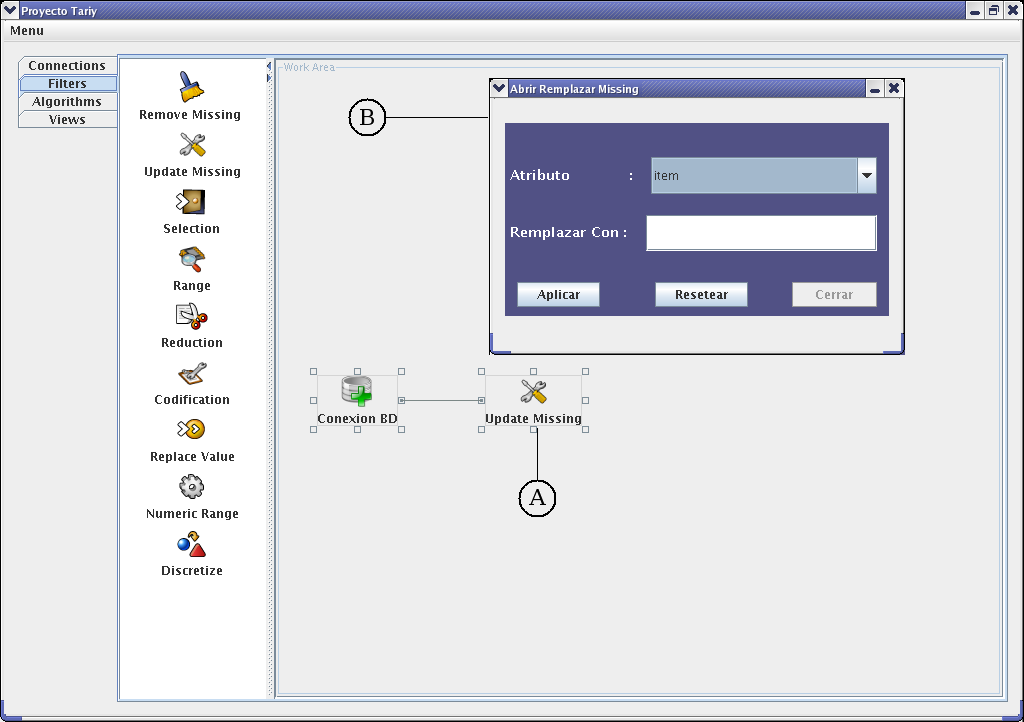
\includegraphics[width=1\textwidth]{images/fi2.png}
\caption{Configuraci\'on filtro Update Missing}
\end{figure}
% TABLA 13
\begin{center}
\begin{tabular}{|p{60mm}|p{60mm}|} \hline
ACCI\'ON DEL ACTOR & RESPUESTA DEL SISTEMA \\ \hline
1. El usuario hace click derecho sobre el filtro A y elige la opci\'on 'Configuraci\'on'& 2. Se muestra B la ventana de configuraci\'on correspondiente al filtro 'Update Missing'. Los campos son: Atributo, en el cual se escribe el nombre del atributo a buscar en el conjunto de datos. Reemplazar con, aqui se escribe el nuevo valor del atributo \\ \hline
\end{tabular}
\end{center}

%------------------------hacer de aqui en adelante------------------------------------------------------------

\newpage
\subsubsection{Configuraci\'on filtro Selection}
\begin{figure}[ht]
\centering
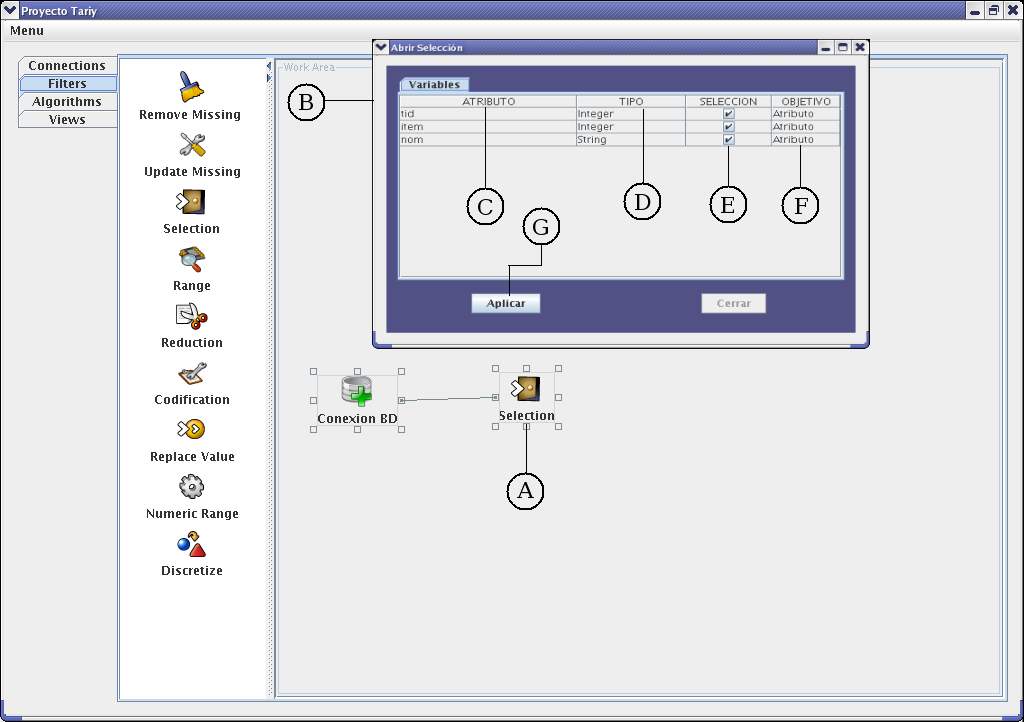
\includegraphics[width=1\textwidth]{images/fi3ver.png}
\caption{Configuraci\'on filtro Selection}
\end{figure}
% TABLA 13
\begin{center}
\begin{tabular}{|p{60mm}|p{60mm}|} \hline
ACCI\'ON DEL ACTOR & RESPUESTA DEL SISTEMA \\ \hline
1. El usuario hace click derecho sobre el filtro A y elige la opci\'on 'Configuraci\'on'& 2. Se muestra B la ventana de configuraci\'on correspondiente al filtro 'Selection'. Los campos son: C: Atributo, en esta grilla se muestran los nombres de los atributos seleccionados. D: Tipo, muestra el tipo de datos de los atributos. E: cajas de verificaci\'on para escoger los atributos a utilizar. F: es posible escoger un atributo clase haciendo click sobre estos campos. Esto es \'util en experimentos de clasificaci\'on. G: el bot\'on 'Aplicar' debe ser precionado para que el filtro sea aplicado. \\ \hline
\end{tabular}
\end{center}
%------------------------hacer de aqui en adelante------------------------------------------------------------

\newpage
\subsubsection{Configuraci\'on filtro Range}
\begin{figure}[ht]
\centering
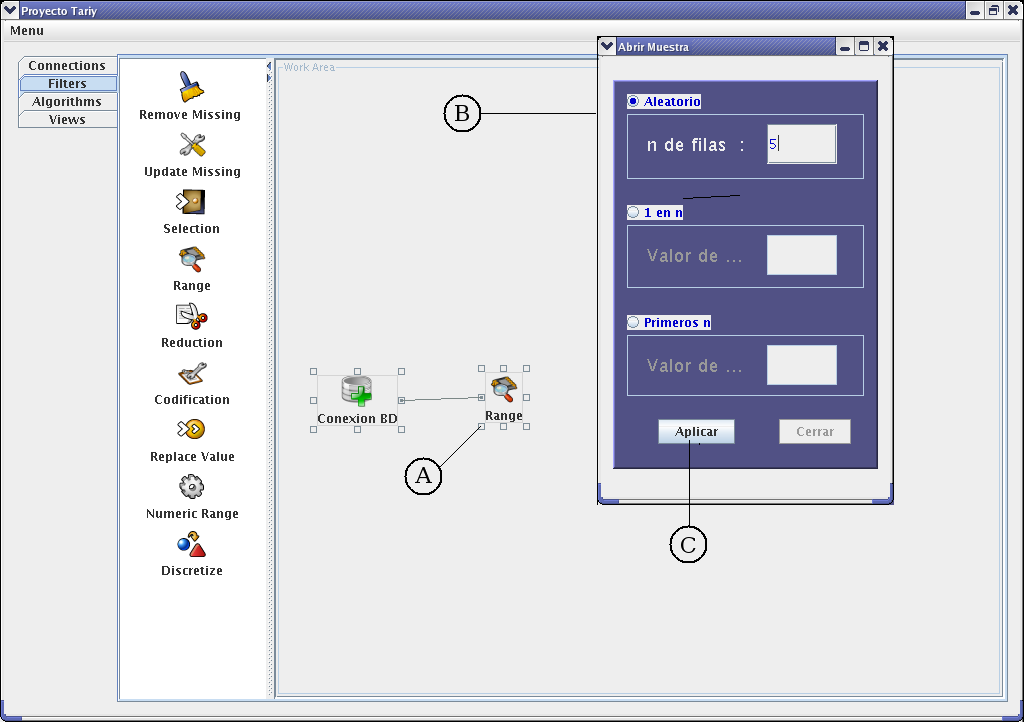
\includegraphics[width=1\textwidth]{images/fi4.png}
\caption{Configuraci\'on filtro Range}
\end{figure}
% TABLA 13
\begin{center}
\begin{tabular}{|p{60mm}|p{60mm}|} \hline
ACCI\'ON DEL ACTOR & RESPUESTA DEL SISTEMA \\ \hline
1. El usuario hace click derecho sobre el filtro A y elige la opci\'on 'Configuraci\'on'& 2. Se muestra B la ventana de configuraci\'on correspondiente al filtro 'Range'. Los campos son:\textbf{Aleatorio}, en donde se escribe el n\'umero \textbf{n} de filas que se desea sean escogidas aleatoriamente. \textbf{1 en n}, donde \textbf{n} es el periodo utilizado para seleccionar los datos a utilizar. \textbf{Primeros n}, donde \textbf{n}es el nmero campos a incluir en la selecci\'on a partir del primero. \\ \hline
\end{tabular}
\end{center}
%------------------------hacer de aqui en adelante------------------------------------------------------------u

\newpage
\subsubsection{Configuraci\'on filtro Reduction}
\begin{figure}[ht]
\centering
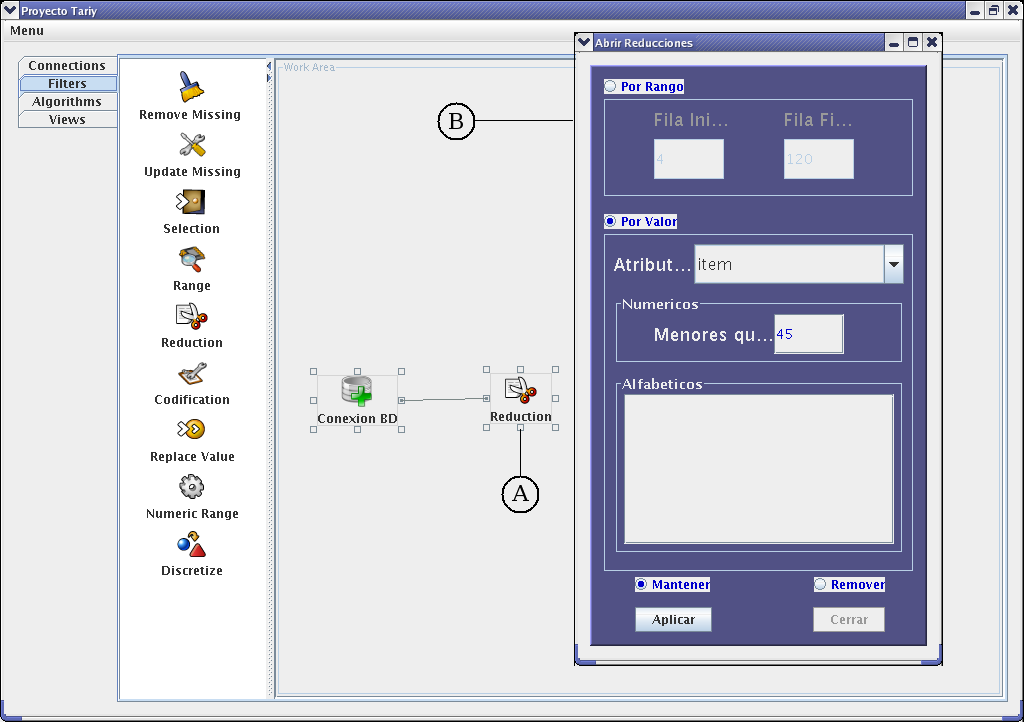
\includegraphics[width=1\textwidth]{images/fi5.png}
\caption{Configuraci\'on filtro Reduction}
\end{figure}
% TABLA 13
\begin{center}
\begin{tabular}{|p{60mm}|p{60mm}|} \hline
ACCI\'ON DEL ACTOR & RESPUESTA DEL SISTEMA \\ \hline
1. El usuario hace click derecho sobre el filtro A y elige la opci\'on 'Configuraci\'on'& 2. Se muestra la ventana B de configuraci\'on correspondiente al filtro 'Reduction'. Los campos son: \textbf{Por rango}, los campos son 'Fila ini cial' donde se escribe la fila a partir de la cual inicia el rango y 'Fila final' que es el l\'imite superior del rango. \textbf{Por Valor:} Se elige el nombre del atributo y luego en caso de que los valores a quitar sean num\'ericos en el campo 'Menores que' se especifica el nmero a partir del cual se hace la reducci\'on. Si el atributo es alfab\'etico se escribe su valor en el \'area de texto y en las casillas de selecci\'on se especifica si ese valor se desea 'Mantener' o 'Remover'. \textbf{Aplicar}: ejecuta el filtro.  \\ \hline
\end{tabular}
\end{center}
%------------------------hacer de aqui en adelante------------------------------------------------------------v

\newpage
\subsubsection{Configuraci\'on filtro Codification}
\begin{figure}[ht]
\centering
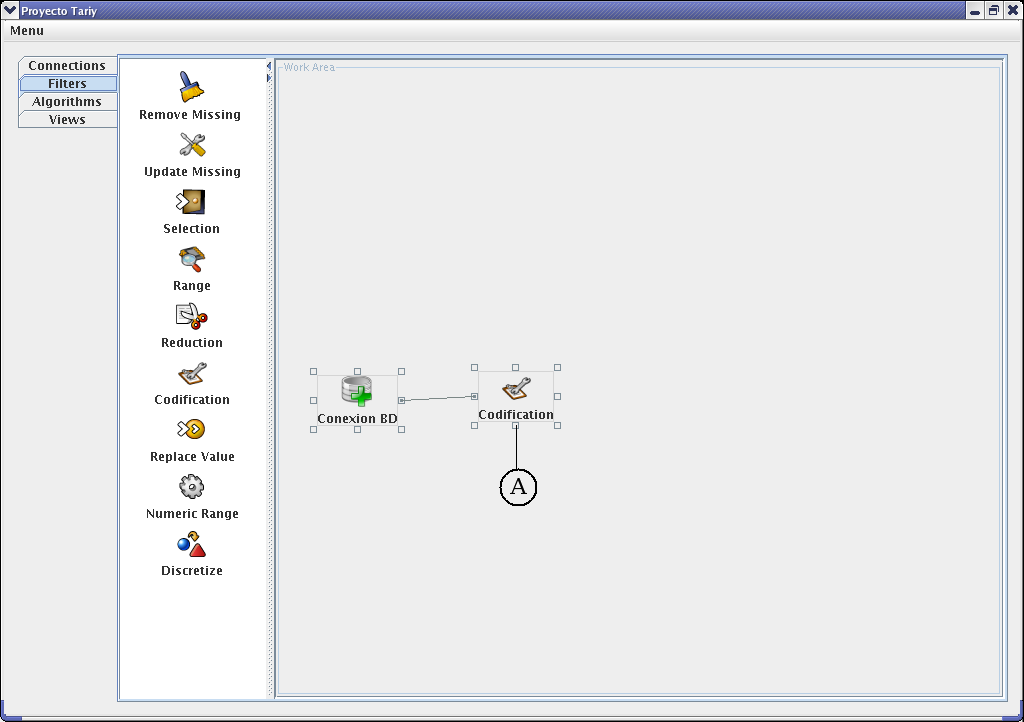
\includegraphics[width=1\textwidth]{images/fi6.png}
\caption{Configuraci\'on filtro Codification}
\end{figure}
% TABLA 13
\begin{center}
\begin{tabular}{|p{60mm}|p{60mm}|} \hline
ACCI\'ON DEL ACTOR & RESPUESTA DEL SISTEMA \\ \hline
1. El usuario hace click derecho sobre el filtro A y elige la opci\'on 'Configuraci\'on'& 2. Se muestra la ventana de configuraci\'on correspondiente al filtro 'Codifcation'. Este filtro no tiene ventana de configuraci\'on. Se aplica para asignar un n\'umero a valores alfab\'eticos\\ \hline
\end{tabular}
\end{center}
%------------------------hacer de aqui en adelante------------------------------------------------------------w

\newpage
\subsubsection{Configuraci\'on filtro Replace Value}
\begin{figure}[ht]
\centering
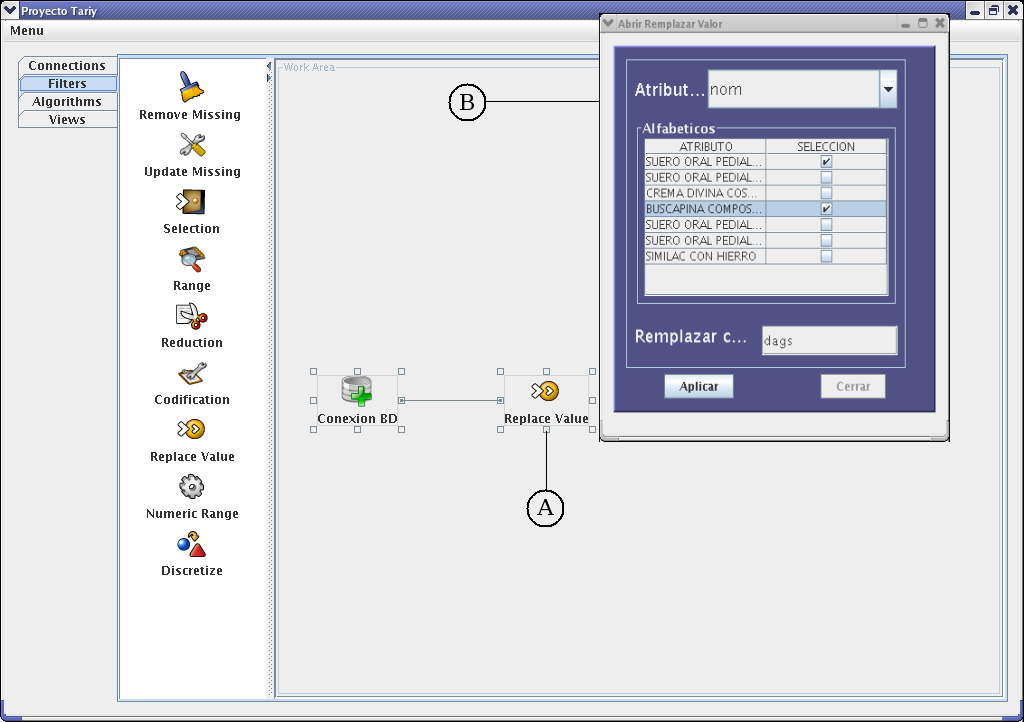
\includegraphics[width=1\textwidth]{images/fi7.png}
\caption{Configuraci\'on filtro Replace Value}
\end{figure}
% TABLA 13
\begin{center}
\begin{tabular}{|p{60mm}|p{60mm}|} \hline
ACCI\'ON DEL ACTOR & RESPUESTA DEL SISTEMA \\ \hline
1. El usuario hace click derecho sobre el filtro A y elige la opci\'on 'Configuraci\'on'& 2. Se muestra la ventana de configuraci\'on correspondiente al filtro 'Replace Value'. Los campos son: Atributo, en el cual se elige el nombre del atributo a buscar en el conjunto de datos. Reemplazar con, aqui se escribe el nuevo valor del atributo. \textbf{Aplicar}: ejecuta el filtro.  \\ \hline
\end{tabular}
\end{center}
%------------------------hacer de aqui en adelante------------------------------------------------------------

\newpage
\subsubsection{Configuraci\'on filtro Numeric Range}
\begin{figure}[ht]
\centering
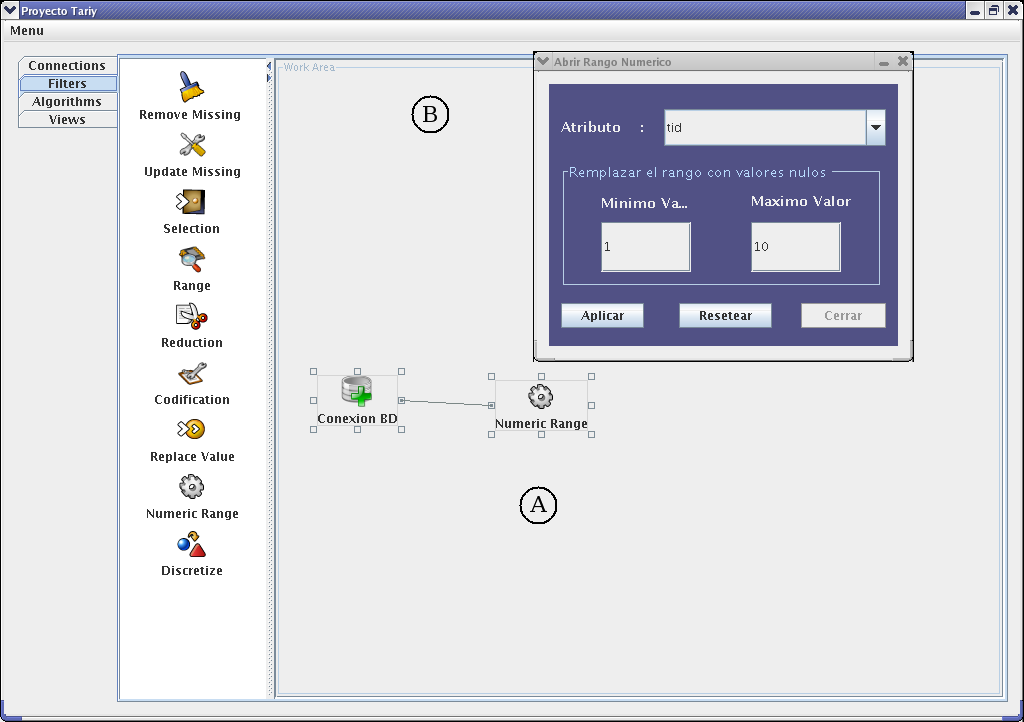
\includegraphics[width=1\textwidth]{images/fi8.png}
\caption{Configuraci\'on filtro Numeric Range}
\end{figure}
% TABLA 13
\begin{center}
\begin{tabular}{|p{60mm}|p{60mm}|} \hline

ACCI\'ON DEL ACTOR & RESPUESTA DEL SISTEMA \\ \hline
1. El usuario hace click derecho sobre el filtro A y elige la opci\'on 'Configuraci\'on'& 2. Se muestra la ventana B de configuraci\'on correspondiente al filtro 'Numeric Range'. Los campos son: \textbf{Atributo}, en el cual se escribe el nombre del atributo a discretizar de tipo num\'erico. \textbf{Reemplazar rango con valores nulos}: aqui es posible especificar un rango de datos que seran convertidos a n\'ulos. \textbf{M\'imimo valor}: l\'imite inferiror del rango. \textbf{M\'inimo valor}: l\'imite superior del rango.  \textbf{Aplicar}: ejecuta el filtro. \textbf{Resetear}: deja los campos en blanco  \\ \hline
\end{tabular}
\end{center}
%------------------------hacer de aqui en adelante------------------------------------------------------------

\newpage
\subsubsection{Configuraci\'on filtro Discretize}
\begin{figure}[ht]
\centering
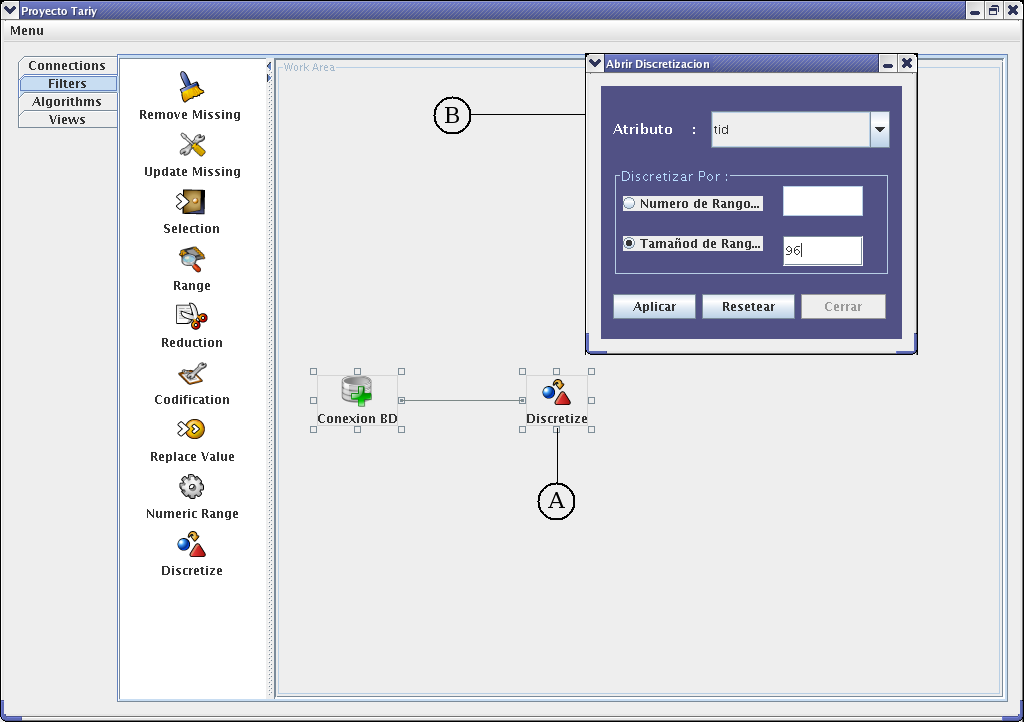
\includegraphics[width=1\textwidth]{images/fi9.png}
\caption{Configuraci\'on filtro Discretize}
\end{figure}
% TABLA 13
\begin{center}
\begin{tabular}{|p{60mm}|p{60mm}|} \hline
ACCI\'ON DEL ACTOR & RESPUESTA DEL SISTEMA \\ \hline
1. El usuario hace click derecho sobre el filtro A y elige la opci\'on 'Configuraci\'on'& 2. Se muestra la ventana B de configuraci\'on correspondiente al filtro 'Discretize'. Los campos son: \textbf{Atributo}, en el cual se escribe el nombre del atributo a discretizar. \textbf{Discretizar por}: 'N\'umero de rango': se puede establecer el n\'umero de rangos a crear. 'Tama\~no del rango': se especifica el tama\~no del rango \textbf{Aplicar}: ejecuta el filtro. \textbf{Resetear}: deja los campos en blanco  \\ \hline
\end{tabular}
\end{center}

\newpage
\subsubsection{Algoritmos}
\begin{figure}[h]
 \centering
 
\includegraphics[width=1\textwidth]{images/a1.png}
 \caption{Algoritmo Apriori}
\end{figure}

\begin{center}
\begin{tabular}{|p{60mm}|p{60mm}|}\hline
ACCI\'ON DEL ACTOR & RESPUESTA DEL SISTEMA \\ \hline
1. Si el usuario quiere minar los datos con Apriori y presiona sobre A (\'Area de opciones), en el icono respectivo.
& 2. En B (\'Area de trabajo) aparece el icono del algoritmo Apriori. \\ \hline
\end{tabular}
\end{center}
\newpage

\subsubsection{Opci\'on Delete}
\begin{figure}[h]
 \centering
 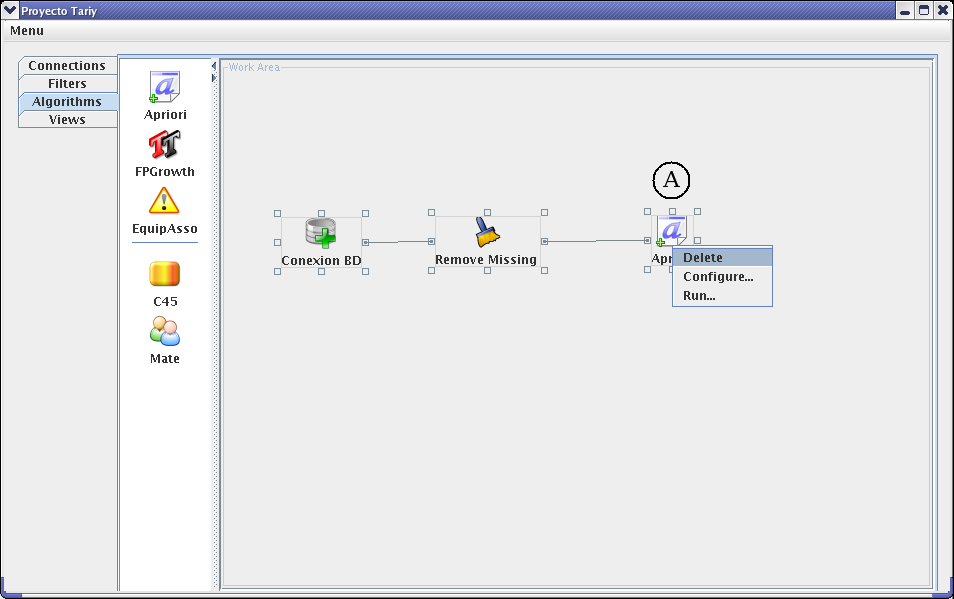
\includegraphics[width=1\textwidth]{images/am1.png}
 \caption{Opci\'on Delete}
\end{figure}

\begin{center}
\begin{tabular}{|p{60mm}|p{60mm}|}\hline
ACCI\'ON DEL ACTOR & RESPUESTA DEL SISTEMA \\ \hline
1. El usuario hace click derecho sobre A: el icono del algoritmo (cualquiera que este sea, Apriori, EquipAsso,
FPGrowth, MateBy o C4.5) y elige la opci\'on delete del men\'u de configuraci\'on.
& 2. El icono del algoritmo es borrado del \'area de trabajo. \\ \hline
\end{tabular}
\end{center}
\newpage

\subsubsection{Opci\'on Configure}
\begin{figure}[h]
 \centering
 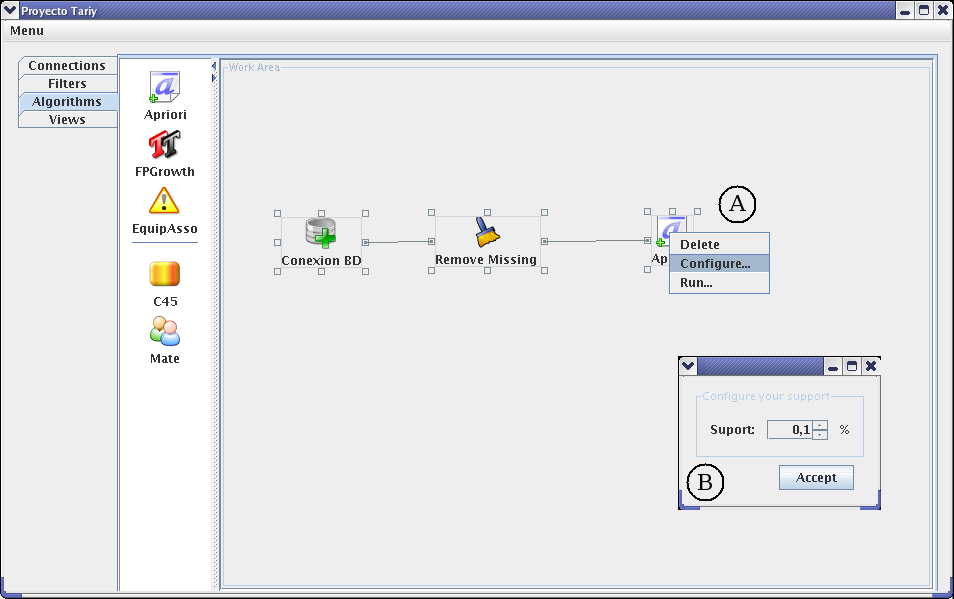
\includegraphics[width=0.9\textwidth]{images/am2.png}
 \caption{Opci\'on Configure}
\end{figure}

\begin{center}
\begin{tabular}{|p{60mm}|p{60mm}|}\hline
ACCI\'ON DEL ACTOR & RESPUESTA DEL SISTEMA \\ \hline
1. El usuario hace click derecho sobre A: el icono del algoritmo (cualquiera que este sea, Apriori, EquipAsso,
FPGrowth, MateBy o C4.5) y elige configurar sus parametros.
& 2. Sobre el \'area de trabajo aparece una ventana B, para que el usuario configure el soporte del algoritmo. \\
\hline
\end{tabular}
\end{center}
\newpage

\subsubsection{Opci\'on Run}
\begin{figure}[h]
 \centering
 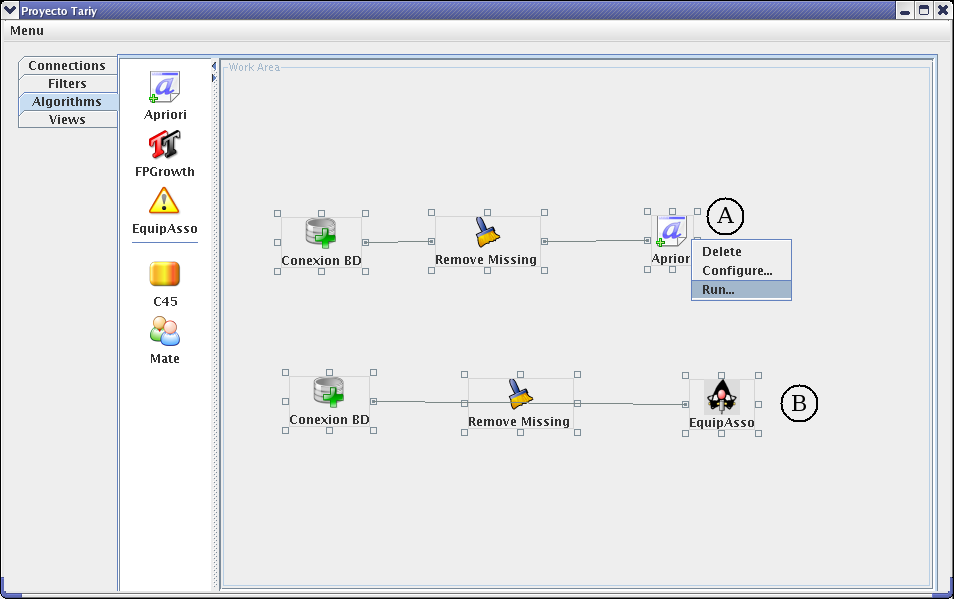
\includegraphics[width=0.9\textwidth]{images/am3.png}
 \caption{Opci\'on Run}
\end{figure}

\begin{center}
\begin{tabular}{|p{60mm}|p{60mm}|}\hline
ACCI\'ON DEL ACTOR & RESPUESTA DEL SISTEMA \\ \hline
1. El usuario hace click derecho sobre A: el icono del algoritmo (cualquiera que este sea, Apriori, EquipAsso,
FPGrowth, MateBy o C4.5) y elige la opci\'on run.
& 2. El icono del algoritmo cambia por una animaci\'on, as\'i como se muestra en B. \\
\hline
\end{tabular}
\end{center}
\newpage

\subsubsection{Algoritmo FPGrowth}
\begin{figure}[h]
 \centering
 
\includegraphics[width=1\textwidth]{images/a2.png}
 \caption{Algoritmo FPGrowth}
\end{figure}

\begin{center}
\begin{tabular}{|p{60mm}|p{60mm}|}\hline
ACCI\'ON DEL ACTOR & RESPUESTA DEL SISTEMA \\ \hline
1. Si el usuario quiere minar los datos con FPGrowth y presiona sobre A (\'Area de opciones), en el icono respectivo.
& 2. En B (\'Area de trabajo) aparece el icono del algoritmo FPGrowth. \\ \hline
\end{tabular}
\end{center}
\newpage

\subsubsection{Algoritmo EquipAsso}
\begin{figure}[h]
 \centering
 
\includegraphics[width=1\textwidth]{images/a3.png}
 \caption{Algoritmo EquipAsso}
\end{figure}

\begin{center}
\begin{tabular}{|p{60mm}|p{60mm}|}\hline
ACCI\'ON DEL ACTOR & RESPUESTA DEL SISTEMA \\ \hline
1. Si el usuario quiere minar los datos con EquipAsso y presiona sobre A (\'Area de opciones), en el icono
respectivo. & 2. En B (\'Area de trabajo) aparece el icono del algoritmo EquipAsso. \\ \hline
\end{tabular}
\end{center}
\newpage

\subsubsection{Algoritmo C4.5}
\begin{figure}[h]
 \centering
 
\includegraphics[width=1\textwidth]{images/a4.png}
 \caption{Algoritmo C4.5}
\end{figure}

\begin{center}
\begin{tabular}{|p{60mm}|p{60mm}|}\hline
ACCI\'ON DEL ACTOR & RESPUESTA DEL SISTEMA \\ \hline
1. Si el usuario quiere minar los datos con C4.5 y presiona sobre A (\'Area de opciones), en el icono respectivo.
& 2. En B (\'Area de trabajo) aparece el icono del algoritmo C4.5. \\ \hline
\end{tabular}
\end{center}
\newpage

\subsubsection{Algoritmo Mate}
\begin{figure}[h]
 \centering
 
\includegraphics[width=1\textwidth]{images/a5.png}
 \caption{Algoritmo Mate}
\end{figure}

\begin{center}
\begin{tabular}{|p{60mm}|p{60mm}|}\hline
ACCI\'ON DEL ACTOR & RESPUESTA DEL SISTEMA \\ \hline
1. Si el usuario quiere minar los datos con Mate y presiona sobre A (\'Area de opciones), en el icono respectivo.
& 2. En B (\'Area de trabajo) aparece el icono del algoritmo Mate. \\ \hline
\end{tabular}
\end{center}
\newpage

\subsubsection{Diagrama de Visualizaci\'on}
\begin{figure}[h]
 \centering
 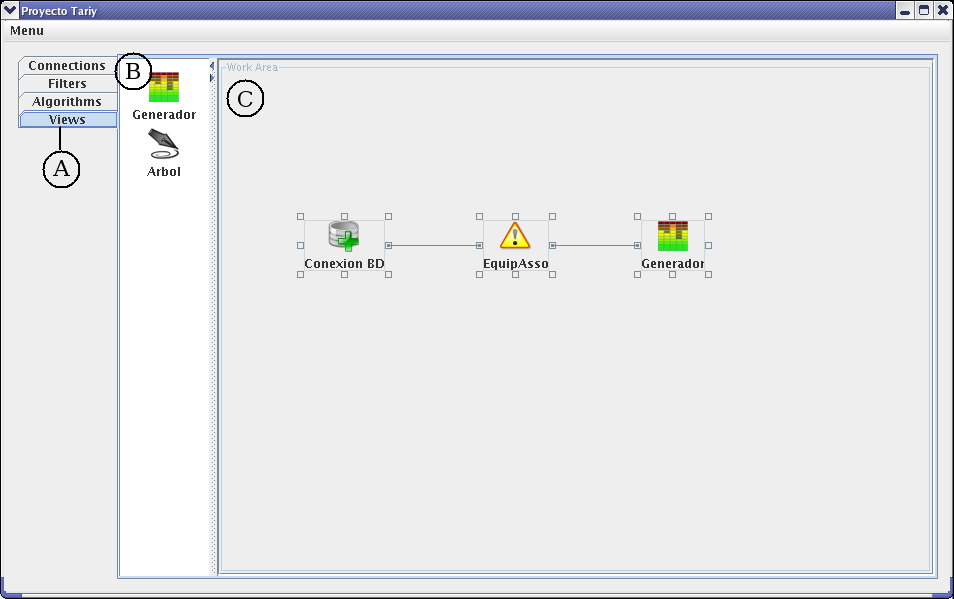
\includegraphics[width=1\textwidth]{images/v01.png}
 \caption{Diagrama de Visualizaci\'on}
\end{figure}

\begin{center}
\begin{tabular}{|p{60mm}|p{60mm}|}\hline
ACCI\'ON DEL ACTOR & RESPUESTA DEL SISTEMA \\ \hline
1. Cuando el usuario ha construido una secuencia de Miner\'ia de Datos, con cualquiera de los algoritmos, en A se
encuentra en la secci\'on de vistas y en B (\'Area de opciones) ha hecho click en el icono generador.
& 2. Entonces en C (\'Area de trabajo) aparece el icono del generador, a trav\'es del cual el usuario puede acceder a las opciones de este m\'odulo. \\ \hline
\end{tabular}
\end{center}
\newpage

\subsubsection{Opci\'on Delete}
\begin{figure}[h]
 \centering
 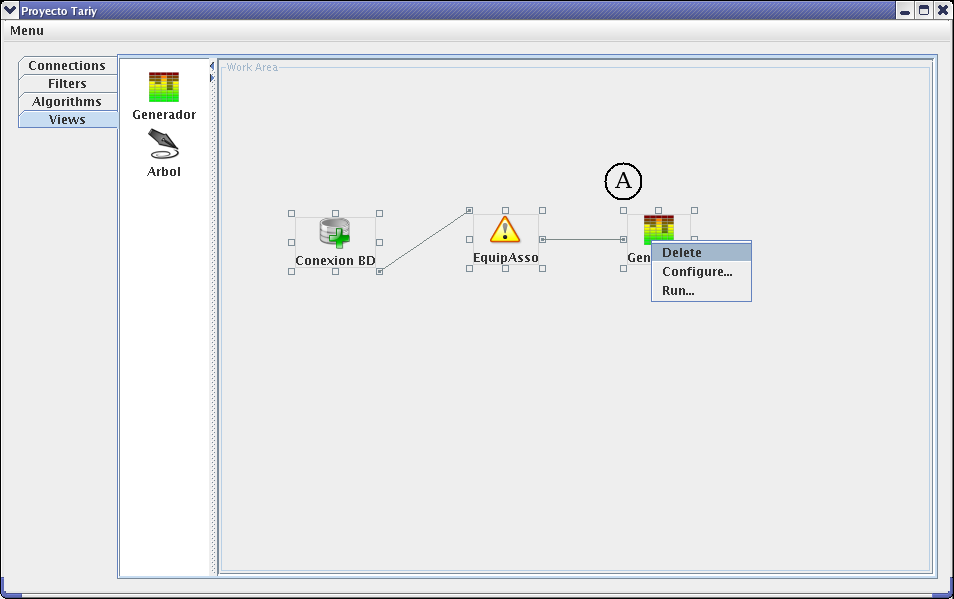
\includegraphics[width=1\textwidth]{images/v0m1.png}
 \caption{Opci\'on Delete}
\end{figure}

\begin{center}
\begin{tabular}{|p{60mm}|p{60mm}|}\hline
ACCI\'ON DEL ACTOR & RESPUESTA DEL SISTEMA \\ \hline
1. El usuario hace click derecho sobre A: el icono generador y elige la opci\'on Delete.
& 2. El icono desaparece del \'area de trabajo, esperando un nuevo icono en la secuencia de Miner\'ia de Datos. \\
\hline
\end{tabular}
\end{center}
\newpage

\subsubsection{Opci\'on Configure}
\begin{figure}[h]
 \centering
 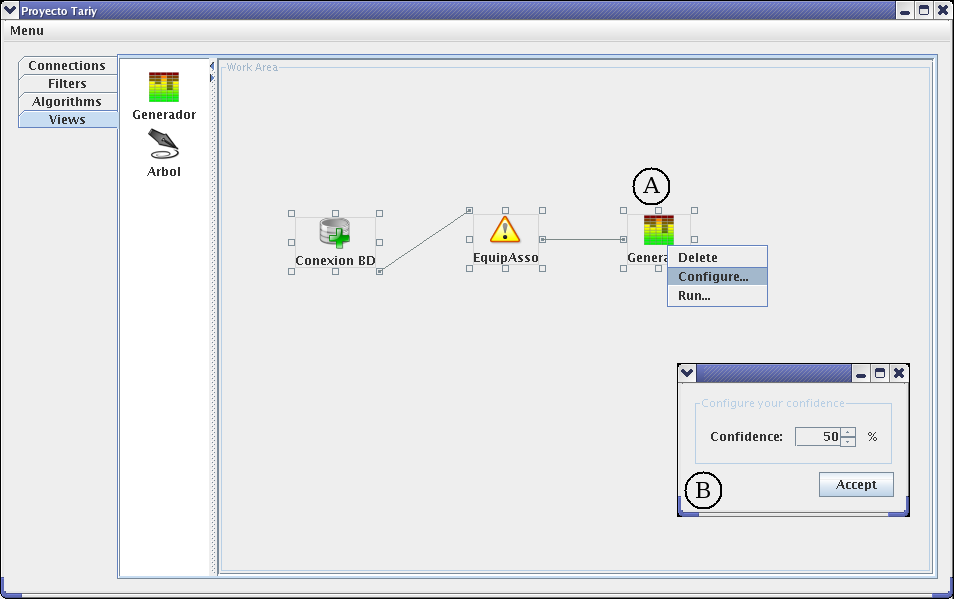
\includegraphics[width=1\textwidth]{images/v0m2.png}
 \caption{Opci\'on Configure}
\end{figure}

\begin{center}
\begin{tabular}{|p{60mm}|p{60mm}|}\hline
ACCI\'ON DEL ACTOR & RESPUESTA DEL SISTEMA \\ \hline
1. El usuario hace click sobre A: el icono del generador y elige configurar sus parametros.
& 2. Sobre el \'area de trabajo aparece una ventana B, para que el usuario configure la confianza con la cual se van a
filtrar las reglas de asociaci\'on. \\ \hline
\end{tabular}
\end{center}
\newpage

\subsubsection{Opci\'on Run}
\begin{figure}[h]
 \centering
 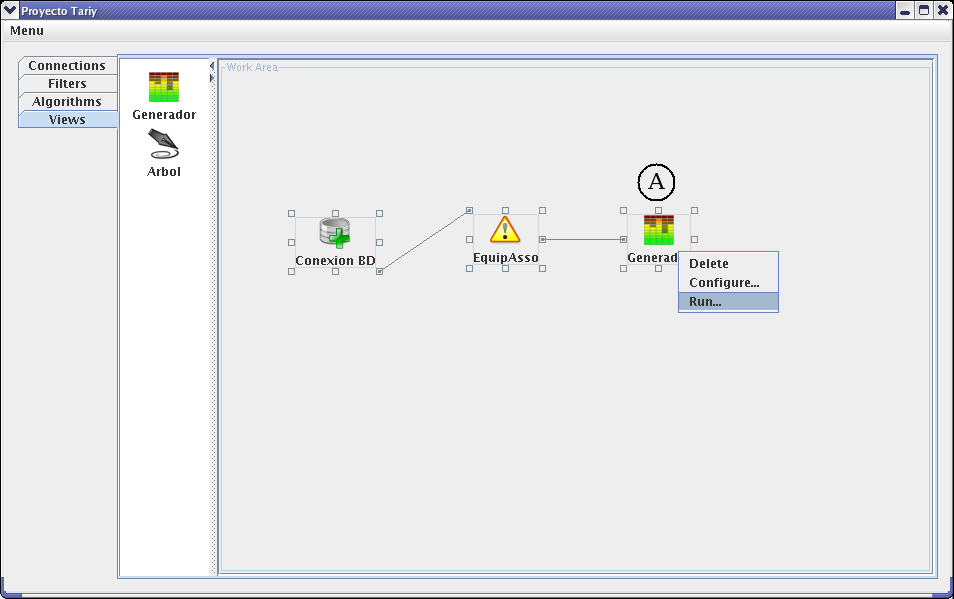
\includegraphics[width=1\textwidth]{images/v0m3.png}
 \caption{Opci\'on Run}
\end{figure}

\begin{center}
\begin{tabular}{|p{60mm}|p{60mm}|}\hline
ACCI\'ON DEL ACTOR & RESPUESTA DEL SISTEMA \\ \hline
1. El usuario hace click derecho sobre A: el icono generador y elige la opci\'on Run.
& 2. En el \'area de trabajo aparece una ventana B, con las reglas obtenidas a partir de los algoritmos de Miner\'ia de
Datos (La cual se explica en la siguiente figura). \\ \hline
\end{tabular}
\end{center}
\newpage

\subsubsection{Visor de Reglas}
\begin{figure}[h]
 \centering
 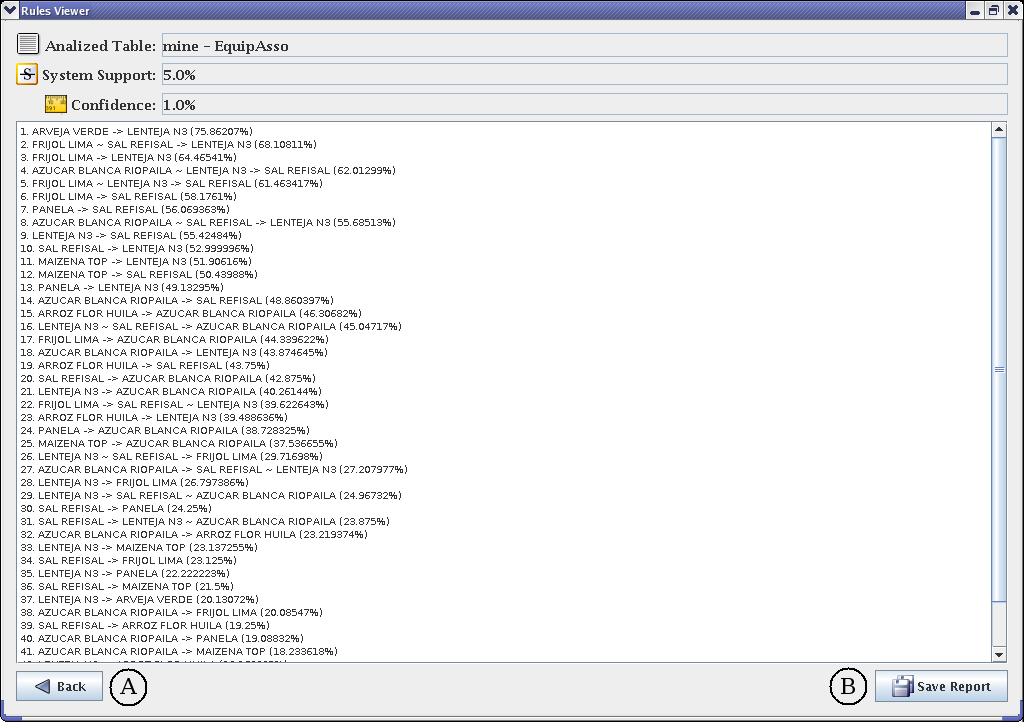
\includegraphics[width=1\textwidth]{images/v0r.png}
 \caption{Visor de Reglas}
\end{figure}

\begin{center}
\begin{tabular}{|p{60mm}|p{60mm}|}\hline
ACCI\'ON DEL ACTOR & RESPUESTA DEL SISTEMA \\ \hline
1. El usuario tiene la opci\'on de hacer click en A, o en B.
& 2. Al hacer click en A, la ventana de reglas desaparece y si hace click en B el usuario tiene la opci\'on de guardar
el reporte de las reglas de asociaci\'on. \\ \hline
\end{tabular}
\end{center}
